\documentclass[10pt,a4paper]{article}

\usepackage{indentfirst}
\usepackage{amsthm,amsfonts,amsmath,amssymb}
\usepackage[brazilian]{babel}
\usepackage[T1]{fontenc}
\usepackage[utf8]{inputenc}
\usepackage{setspace}
\usepackage[usenames,dvipsnames]{xcolor} 
\usepackage{pgf,tikz}
\usepackage{float}
\usepackage{graphicx}
\usepackage{subfigure}
\usepackage{wrapfig}
\usepackage{multirow}
\usepackage{changepage}
\usepackage{geometry}
\usepackage[pdftex]{hyperref}
\usepackage{listings}
\usepackage[normalem]{ulem}
\usepackage{enumitem}
\usepackage{booktabs}
\usepackage{multirow,array,varwidth}
\usepackage{tabularx}
\usepackage{makeidx}
\usepackage[nottoc]{tocbibind}
\usepackage{caption}
\usepackage{longtable}
\usepackage{tabularx}
\usepackage{lscape}
\usepackage{etoolbox}
\usepackage{calc}
\geometry{a4paper,inner=2.0cm,outer=2.0cm,top=2.0cm,bottom=2.0cm}
\setenumerate[1]{label=\thesubsection.\arabic*.}
\setenumerate[2]{label*=\arabic*.}

\newcommand*\NewPage{\newpage\null\thispagestyle{empty}\newpage}
\newcommand{\pr}{\hspace*{0.6cm}}
\newcommand{\vesp}{\vspace*{.3cm}}

\setlength{\columnsep}{1cm}
\addto\captionsbrazilian{% Replace "english" with the language you use
  \renewcommand{\contentsname}%
    {Tabela de Conteúdo}%
}
\definecolor{gray}{rgb}{0.4,0.4,0.4}
\definecolor{darkblue}{rgb}{0.0,0.0,0.6}
\definecolor{cyan}{rgb}{0.0,0.6,0.6}

\lstset{
  basicstyle=\ttfamily,
  columns=fullflexible,
  showstringspaces=false,
  commentstyle=\color{gray}\upshape
}

\lstdefinelanguage{XML}
{
  morestring=[b]",
  morestring=[s]{>}{<},
  morecomment=[s]{<?}{?>},
  stringstyle=\color{black},
  identifierstyle=\color{darkblue},
  keywordstyle=\color{red},
  morekeywords={xmlns,version,type,encoding,href}% list your attributes here
}

\begin{document}

\thispagestyle{empty}
\begin{center}
	UNIVERSIDADE DE SÃO PAULO – USP
	
	INSTITUTO DE CIÊNCIAS MATEMÁTICAS E DE COMPUTAÇÃO
	
	DEPARTAMENTO DE SISTEMAS DE COMPUTAÇÃO
	
	\vspace{7cm}
	
	\Large{\textbf{Relatório Trabalho 2}}\\
	\small{\textbf{Organização de Computadores Digitais}}
	
	\vspace{6cm}
	
	Adams Vietro Codignotto da Silva - $6791943$ \\ 
	Gabriel Estrela - $8124138$\\
	Luiz Eduardo Dorici - $4165850$ \\
	Maiser J. Alves	- $6309717$\\
	
	
	
	\vspace{6cm}
	
	São Carlos
	
	2015
\end{center}

\NewPage
\pagenumbering{arabic}

\tableofcontents

\newpage

\section{Introdução}
Para este trabalho, foi utilizado o simulador de memória \textit{cache Amnesia}, disponibilizado pela professora. Este simulador possui as opções de variar praticamente qualquer combinação de memória aprendida nesta disciplina, através de arquivos \textit{xmls}, os quais representam  as arquiteturas desejadas, e os arquivos \textit{trace}, que representam as instruções dadas. Estas instruções são divididas entre escrita, leitura ou busca.

\section{Arquivos trace}
Os arquivos trace representam 70 instruções. Foram criados 4 arquivos, seguindo os princípios de localidade espacial, temporal, todos os princípios e nenhum dos princípios. Eles estão neste relatório, e também estão disponíveis em anexo.

\subsection{Princípio Localidade Espacial}
Para este princípio, foi gerado um arquivo em que os acessos são seqüenciais, porém separados por um \textit{gap}.

\begin{table}[H]
\centering
\begin{tabularx}{\textwidth}{*{10}{>{\centering\arraybackslash}X|}}
1 2 & 0 34 & 2 4c & 1 65 & 2 89 & 2 8d & 2 a0 & 0 c0 & 1 cb & 2 e5 \\
2 15 & 2 30 & 2 51 & 2 65 & 2 87 & 2 93 & 1 a2 & 2 c2 & 2 ca & 2 ef \\
2 16 & 1 36 & 2 56 & 2 6a & 2 8b & 2 99 & 2 a7 & 2 c0 & 2 d6 & 2 f0 \\
2 18 & 2 3f & 0 59 & 2 6c & 2 8c & 2 99 & 2 ab & 2 bf & 2 d7 & 2 ee \\
2 25 & 2 42 & 2 61 & 2 6e & 2 89 & 2 99 & 2 b2 & 2 c8 & 2 d9 & 2 f2 \\
2 23 & 2 47 & 2 62 & 2 73 & 2 91 & 2 9d & 2 b7 & 2 ca & 2 dd & 2 f8 \\
2 2a & 2 4e & 2 5e & 2 85 & 0 93 & 2 9c & 2 ba & 2 d0 & 2 da & 0 ff \\
\end{tabularx}
\end{table}
\subsection{Princípio Localidade Temporal}
Foi gerado um arquivo em que a porcentagem de se usar um bloco já utilizado aumenta com o passar do tempo. Todas as seguintes tabelas de \textit{trace} devem ser lidas por coluna, e não por linha.
\begin{table}[H]
\centering
\begin{tabularx}{\textwidth}{*{10}{>{\centering\arraybackslash}X|}}
1 12c & 0 c & 2 8 & 2 8e & 0 5a & 2 4a & 1 4a & 2 c5 & 2 c & 2 c8 \\
0 12c & 2 4a & 2 4a & 1 c & 2 c8 & 1 4a & 2 5a & 2 8 & 2 5a & 2 8 \\
2 c8 & 2 e9 & 2 36 & 2 c & 2 36 & 2 8 & 2 12c & 0 c5 & 1 e9 & 0 12c \\
2 5a & 2 12c & 2 12c & 2 4a & 2 c & 2 8e & 0 5a & 2 4a & 2 36 & 2 5a \\
2 e9 & 2 4a & 2 e9 & 2 12c & 2 8 & 2 8 & 2 c8 & 2 8e & 2 c & 2 e9 \\
2 5a & 1 c & 2 c5 & 2 c5 & 2 c8 & 2 c8 & 2 8 & 2 e9 & 2 c8 & 2 8e \\
2 5a & 2 c & 2 e9 & 2 4a & 2 36 & 2 e9 & 2 c8 & 2 c & 2 c5 & 2 c5 \\
\end{tabularx}
\end{table}
\subsection{Princípio Localidade Espacial e Temporal}
Foram gerados vários acessos em um curto intervalo de endereço, assim forçando os dois princípios a serem ativos.

\begin{table}[H]
\centering
\begin{tabularx}{\textwidth}{*{10}{>{\centering\arraybackslash}X|}}
2 53 & 2 56 & 2 50 & 0 57 & 2 54 & 0 55 & 2 53 & 2 53 & 0 50 & 0 52 \\
2 59 & 2 50 & 2 59 & 2 55 & 2 56 & 2 50 & 0 52 & 1 53 & 2 56 & 2 59 \\
2 59 & 2 52 & 2 51 & 2 59 & 1 57 & 2 59 & 2 51 & 2 58 & 2 59 & 2 55 \\
2 59 & 2 59 & 2 57 & 1 58 & 2 56 & 2 54 & 2 58 & 2 54 & 1 51 & 2 55 \\
2 58 & 2 51 & 2 54 & 2 52 & 2 56 & 2 53 & 2 56 & 2 55 & 2 59 & 0 58 \\
0 50 & 1 59 & 2 53 & 2 54 & 2 57 & 2 52 & 2 53 & 2 54 & 2 51 & 2 51 \\
2 51 & 1 58 & 2 51 & 2 52 & 1 57 & 2 57 & 2 50 & 2 52 & 2 59 & 2 56 \\
\end{tabularx}
\end{table}
\subsection{Nenhum Princípio}
Através de um gerador aleatório, criou-se este \textit{trace}, não respeitando nenhum princípio de localidade.

\begin{table}[H]
\centering
\begin{tabularx}{\textwidth}{*{10}{>{\centering\arraybackslash}X|}}
2 ed & 2 2c & 2 8e & 2 e8 & 2 12 & 1 d6 & 2 99 & 2 90 & 2 d & 2 75 \\
2 5f & 1 c1 & 2 2 & 1 5a & 0 5c & 1 a3 & 2 73 & 2 6f & 2 bd & 0 4f \\
2 b6 & 2 c3 & 0 9a & 2 76 & 2 39 & 0 40 & 2 53 & 0 cf & 1 e4 & 2 63 \\
0 db & 2 6d & 2 ab & 2 3a & 2 a2 & 2 4e & 0 17 & 2 2c & 2 ff & 2 30 \\
2 5d & 2 90 & 2 db & 2 51 & 2 d8 & 2 a2 & 2 8d & 2 49 & 2 6a & 2 e0 \\
2 b3 & 1 36 & 2 51 & 2 d4 & 2 92 & 2 9e & 2 17 & 2 40 & 2 a2 & 2 fc \\
2 a & 2 c3 & 2 4e & 2 25 & 2 40 & 2 70 & 2 2a & 1 a5 & 2 83 & 1 d0 \\
\end{tabularx}
\end{table}
\section{Configurações das arquiteturas}
Foram criadas 10 configurações, que além de estarem neste relatório, estão também em anexo. Note que, todas são variações de apenas um parâmetro da arquitetura base, como foi especificado no enunciado do trabalho.
\subsection{Arquitetura Base}
\lstinputlisting[language=XML]{arqBase.xml}
\subsection{Arquitetura 2 Words}
\lstinputlisting[language=XML]{arq2Words.xml}
\subsection{Arquitetura 4 Words}
\lstinputlisting[language=XML]{arq4Words.xml}
\subsection{Arquitetura Duas Caches Unified}
\lstinputlisting[language=XML]{arqDuasCaches.xml}
\subsection{Arquitetura Cache Splitted}
\lstinputlisting[language=XML]{arqDuasSplit.xml}
\subsection{Arquitetura Associtivadade 4}
\lstinputlisting[language=XML]{arqAssociativity4.xml}
\subsection{Arquitetura Associtivadade 32}
\lstinputlisting[language=XML]{arqAssociativity32.xml}
\subsection{Arquitetura LRU}
\lstinputlisting[language=XML]{arqLRU.xml}
\subsection{Arquitetura Tamanho 64}
\lstinputlisting[language=XML]{arqTam64.xml}
\subsection{Arquitetura Tamanho 128}
\lstinputlisting[language=XML]{arqTam128.xml}
\section{Gráficos e Análise dos Gráficos}
Para os gráficos, escolhemos fazer uma comparação entre cada princípio com as variações de caches.
\subsection{Princípio Localidade Espacial}
\vspace{-1.5cm}
\begin{minipage}[H]{.3\textwidth}
\begin{table}[H]
  \centering
    \begin{tabularx}{\textwidth}{>{\centering}m{\widthof{arqAssociativity32}+2mm}|>{\centering\arraybackslash}m{\widthof{Porcentagem}+2mm}}
	\multirow{2}{*}{Arquitetura} & Porcentagem\\
		&Hit/Rate\\
    \midrule
 arqBase & 10\% \\
 arq2Words & 17,14\% \\
 arq4Words & 35,71\% \\
 arqAssociativity4 & 10\% \\
 arqAssociativity32 & 10\% \\
 arqDuasCachesL1 & 10\% \\
 arqDuasCachesL2 & 7.3\% \\
 arqDuasSplit & 6.66\% \\
 arqLRU & 10\% \\
 arqTam64 & 10\% \\
 arqTam128 & 10\% \\
    \bottomrule
    \end{tabularx}
\end{table}
\end{minipage}
\hspace{0.1cm}
\begin{minipage}[H]{.68\textwidth}
\begin{figure}[H]
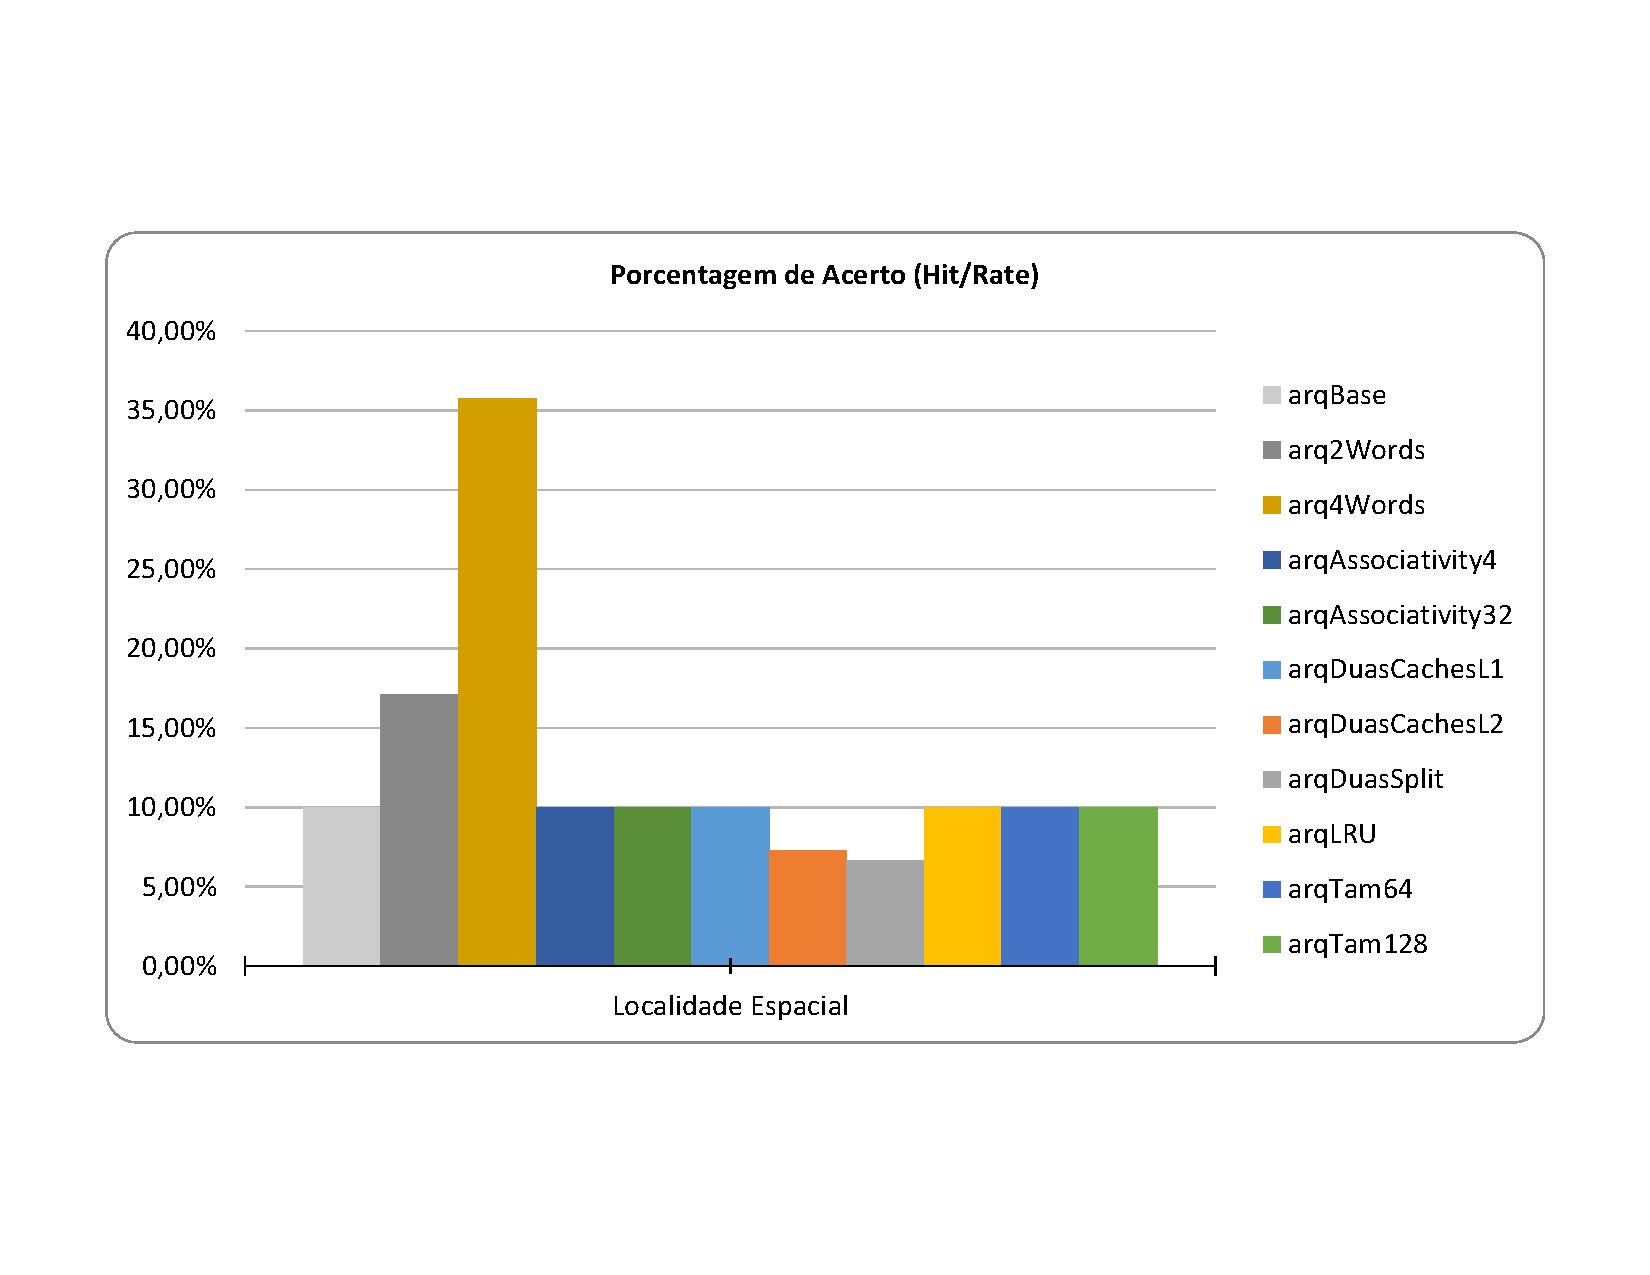
\includegraphics[width=\textwidth]{Localidade.pdf}
\end{figure}
\end{minipage}%
\vspace{-1cm}
\subsubsection{Relação da taxa de acerto (hit rate) com o tamanho da cache}
O principio de localidade espacial diz que ao acessarmos uma posição da memoria primaria temos grandes chances de acessar uma posição próxima a ela, nesse caso o tamanho da memoria pouco influencia pois um bloco de uma única terá miss ao tentar recuperar um dado próximo ao dado já existente na cache.
\subsubsection{Relação da taxa de acerto (hit rate) com o tamanho do bloco}
No caso do aumento do bloco verificamos um aumento no hit rate pois quando carregamos um bloco na cache com mais de uma palavra, também carregamos as palavras próximas a palavra que vamos utilizar, e isso segundo o principio de localidade espacial aumenta o hit rate, ou seja, quando acessamos uma palavra temos grandes chances de acessar uma palavra próxima a ela e quanto maior o numero de palavras por bloco maior as chances de acertarmos ao procurar por elas.
\subsubsection{Relação da taxa de acerto (hit rate) com o nível de associatividade}
No caso de cache associativa não percebemos mudança no hit rate pois sem mudança no tamanho do bloco as chances de encontrarmos uma palavra próxima a palavra que utilizamos em algum momento anterior não aumentam, dessa forma sempre que procuramos uma palavra nova, mesmo que próxima a uma palavra anterior, ela precisa ser carregada na cache novamente e caso a cache esteja cheia, alguma posição dela deve ser liberada, mesmo que seja uma posição contendo um dado próximo ao dado recuperado.
\subsubsection{Relação da taxa de acerto (hit rate) com o algoritmo de substituição}
Não verificamos mudança no hit rate dos algoritmos de substituição pois sem o aumento do bloco da cache não aumentamos o hit rate para o principio de localidade espacial.
\subsubsection{Relação da taxa de acerto (hit rate) com o número de caches}
Podemos verificar que para a arquitetura utilizada na cache de dois níveis, tivemos uma queda no hit rate da cache L2, porem não é significativo para avaliar o principio de localidade espacial, no caso da cache splited também tivemos diminuição do hit rate para essa arquitetura, dessa forma notamos que o hit rate não aumentou pois não ouve aumento do numero de palavras por bloco.
\subsubsection{Análise do Gráfico}
Analisando o gráfico podemos verificar que o hit rate com relação ao aumento do tamanho do bloco na cache, o que já era esperado utilizando o principio de localidade espacial.
\subsection{Princípio Localidade Temporal}%
\vspace{-4.5cm}
\begin{minipage}[H]{.3\textwidth}
\begin{table}[H]
  \centering
     \begin{tabularx}{\textwidth}{>{\centering}m{\widthof{arqAssociativity32}+2mm}|>{\centering\arraybackslash}m{\widthof{Porcentagem}+2mm}}
	\multirow{2}{*}{Arquitetura} & Porcentagem\\
		&Hit/Rate\\
    \midrule
    arqBase & 5,86\% \\
    arq2Words & 5,14\% \\
    arq4Words & 3,71\% \\
    arqAssociativity4 & 8,57\% \\
    arqAssociativity32 & 8,57\% \\
    arqDuasCachesL1 & 2,75\% \\
    arqDuasCachesL2 & 5,17\% \\
    arqDuasSplit & 5,52\% \\
    arqLRU & 5,86\% \\
    arqTam64 & 7,14\% \\
    arqTam128 & 8,57\% \\
    \end{tabularx}%
\end{table}%
\end{minipage}
\hspace{0.1cm}
\begin{minipage}[H]{.68\textwidth}
\begin{figure}[H]
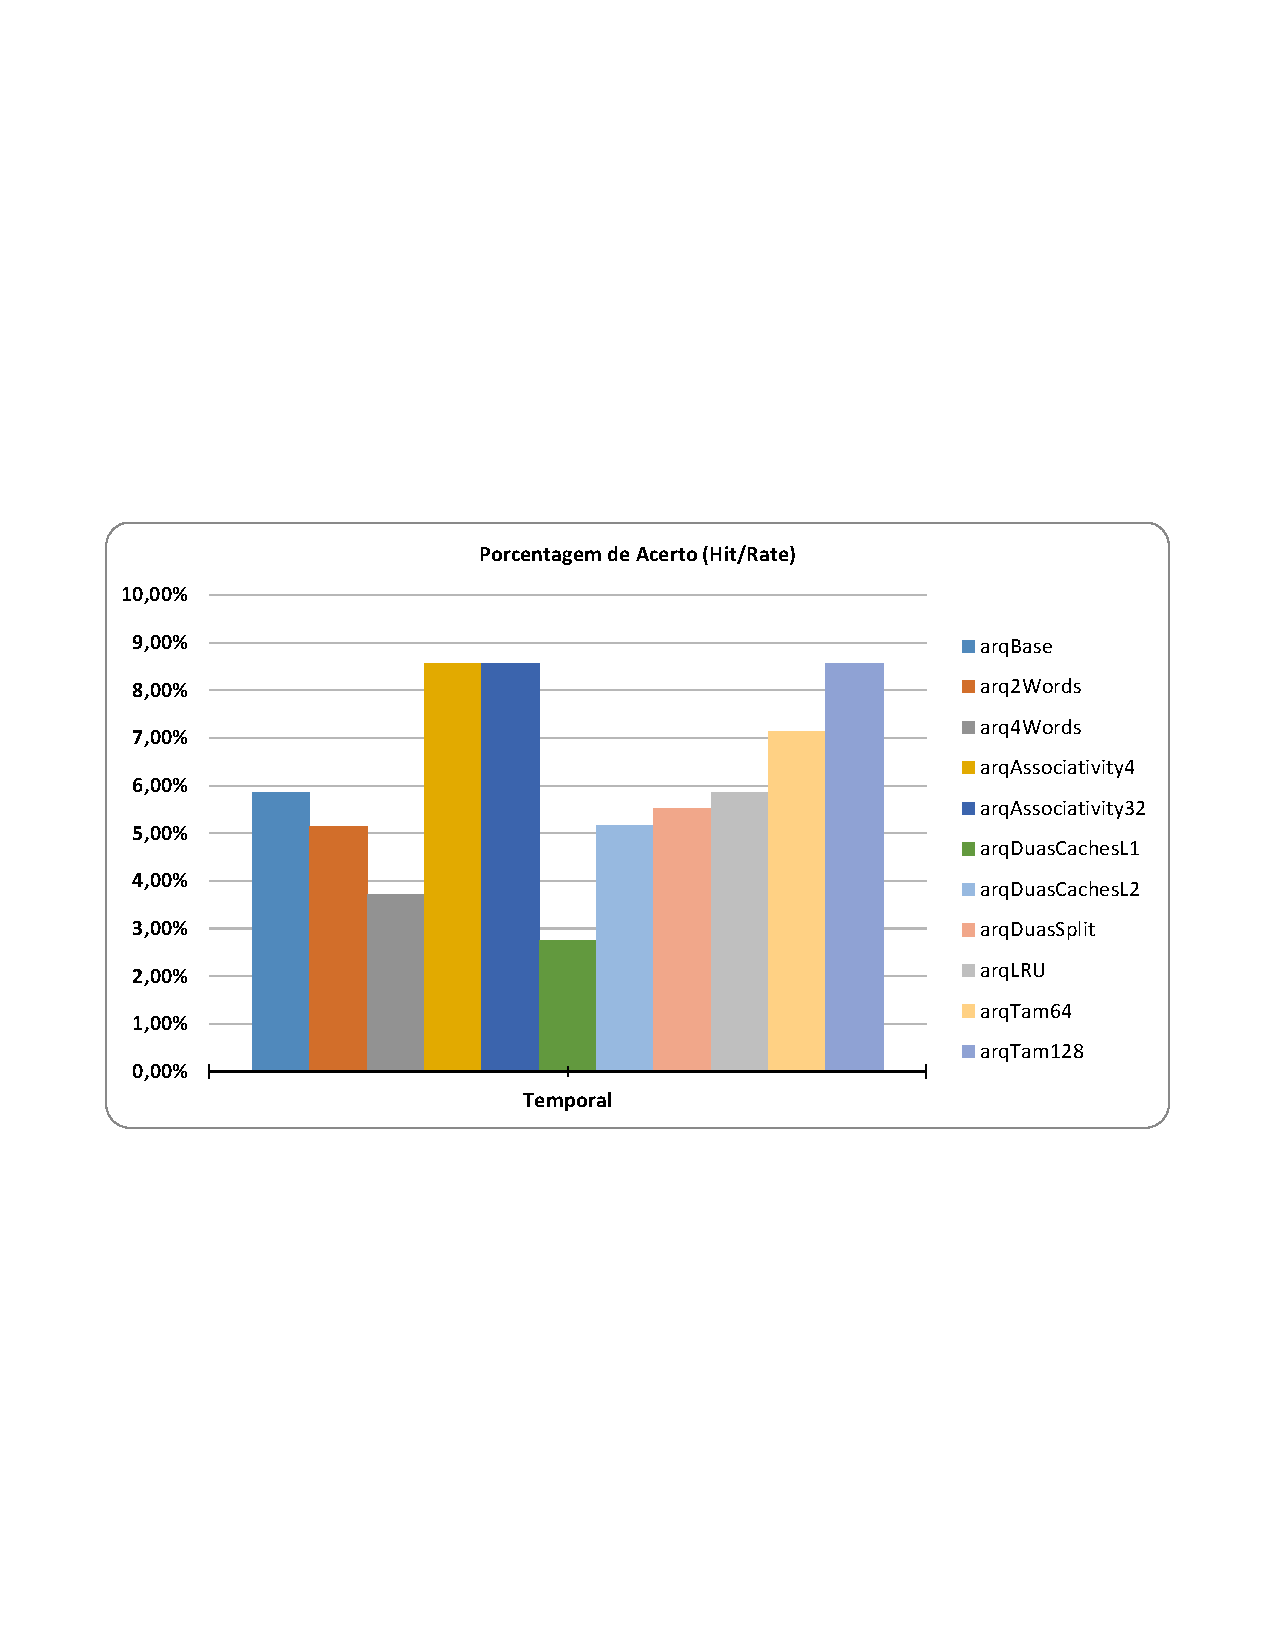
\includegraphics[width=\textwidth]{Temporal.pdf}
\end{figure}
\end{minipage}
\vspace{-4.5cm}
\subsubsection{Relação da taxa de acerto (hit rate) com o tamanho da cache}
O trace baseado no princípio de localidade temporal respeita a ideia de que uma instrução recentemente utilizada será utilizada novamente em breve com probabilidade alta, sendo assim espera-se uma variação na taxa de acerto de acordo com o tipo de cache utilizada.
\subsubsection{Relação da taxa de acerto (hit rate) com o tamanho do bloco}
Nota-se no trace temporal que o tamanho da cache influencia no aumento do hit rate, uma vez que se garante a repetição de um acesso em uma posição com o dado procurado. Como a ram possui 256 palavras, e a chance de se acessar uma mesma palavra duas vezes é alta no trace temporal, o aumento da cache altera o resultado.
\subsubsection{Relação da taxa de acerto (hit rate) com o nível de associatividade}
A diminuição de hit rate para 4 palavras acontece apenas pelo fato de diminuirmos a quantidade de blocos na ram o que faz com que a cache seja modificada com maior frequência. Nota-se que para 2 palavras não houve uma queda tão significativa pois como existe mais blocos em relação à anterior, existe uma probabilidade menor de a cache ter que sobrescrever um dado.
\subsubsection{Relação da taxa de acerto (hit rate) com o algoritmo de substituição}
Era de se esperar que para associatividade maior houvesse uma taxa maior de acertos, uma vez que a cache ira possuir mais blocos por conjunto, assim tendo uma maior quantidade de informação. Porém nota-se que quanto mais blocos por conjunto a partir de 4, o hit rate mostra que o comportamento assintótico desta variação tende a 85.71, isso ocorre porque com k igual a 4 podemos representar a memória principal dentro da cache facilmente.  
\subsubsection{Relação da taxa de acerto (hit rate) com o número de caches}
Como foi pedido que as comparações fossem feitas em relação a arquitetura base, é de se esperar que a mudança na política de substituição não altere a taxa de hit rate, uma vez que o mapeamento direto (escolhido como base), não muda pois já é substituído o bloco que resulta da equação $i = j mod m$.
\subsection{Princípio Localidade Espacial e Temporal}
\vspace{-1.5cm}
\begin{minipage}[H]{.3\textwidth}
\begin{table}[H]
  \centering
    \begin{tabularx}{\textwidth}{>{\centering}m{\widthof{arqAssociativity32}+2mm}|>{\centering\arraybackslash}m{\widthof{Porcentagem}+2mm}}
	\multirow{2}{*}{Arquitetura} & Porcentagem\\
		&Hit/Rate\\
    \midrule
	 arq2Words & 92,87\% \\
     arq4Words & 95,71\% \\
     arqAssociativity4 & 85,71\% \\
     arqAssociativity32 & 85,71\% \\
     arqDuasCachesL1 & 85,71\% \\
     arqDuasCachesL2 & 41,18\% \\
     arqDuasSplit & 82,14\% \\
     arqLRU & 85,71\% \\
     arqTam64 & 85,71\% \\
     arqTam128 & 85,71\% \\

    \bottomrule
    \end{tabularx}
\end{table}
\end{minipage}
\hspace{0.1cm}
\begin{minipage}[H]{.68\textwidth}
\begin{figure}[H]
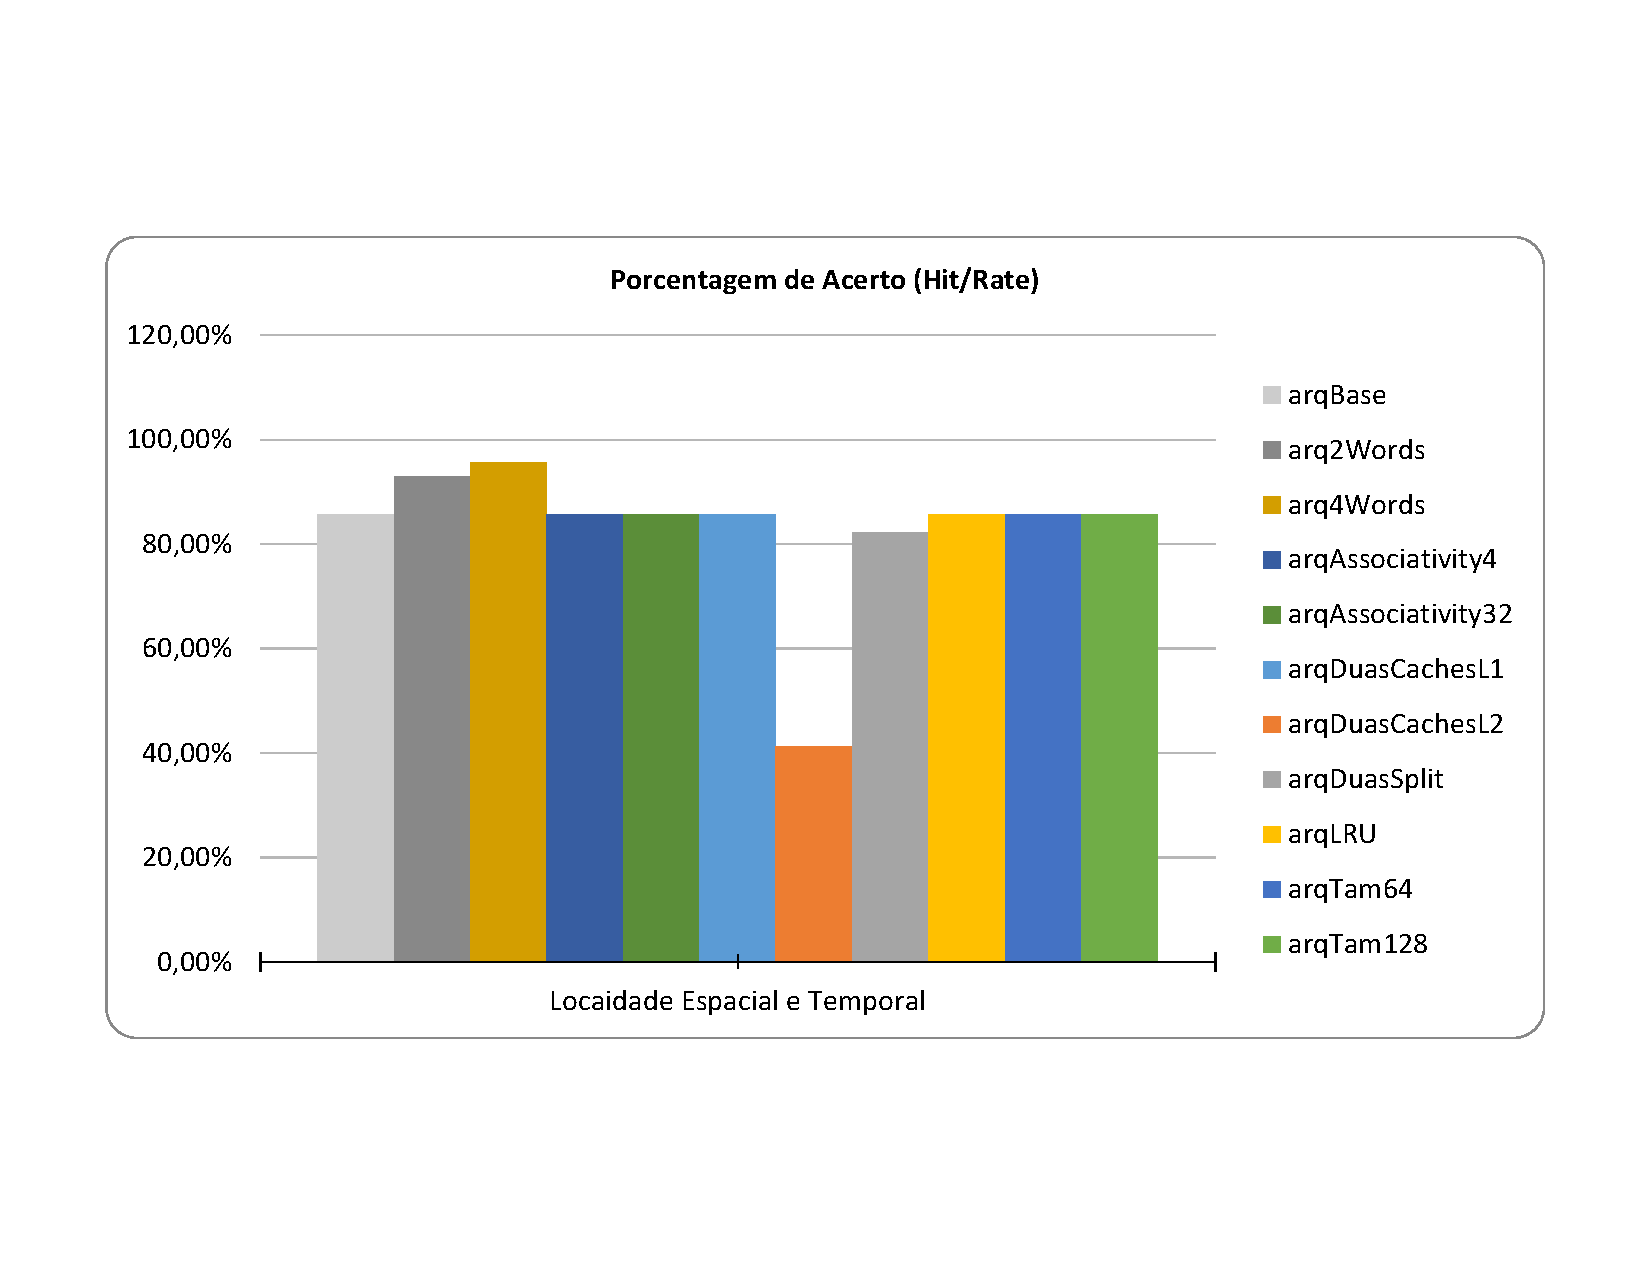
\includegraphics[width=\textwidth]{LocalidadeETemporal.pdf}
\end{figure}
\end{minipage}
\vspace{-1.5cm}
\subsubsection{Relação da taxa de acerto (hit rate) com o tamanho da cache}
A relação da taxa de acerto (hit rate) não aumenta conforme aumentamos o tamanho da cache. Basta olhar para os resultados das simulações das arquiteturas \textit{arqTam64} e \textit{arqTam128} onde é aumentado o tamanho da cache mas a taxa de acerto não varia.
\subsubsection{Relação da taxa de acerto (hit rate) com o tamanho do bloco}
A relação da taxa de acerto (hit rate) aumentou significativamente com o aumento do número do words por bloco (tamanho do bloco). Basta olhar o resultado das simulações \textit{arq2Words} e \textit{arq4Words}. Portanto aumentar o número de words por bloco melhora muito a taxa de acerto.
\subsubsection{Relação da taxa de acerto (hit rate) com o nível de associatividade}
Não houve aumento da taxa com o aumento do grau de associatividade. Portanto, não há um impacto grande do grau de associatividade na taxa de acerto para este arquivo de trace.
\subsubsection{Relação da taxa de acerto (hit rate) com o algoritmo de substituição}
A taxa não aumenta com a mudança do algoritmo de substituição. Basta olhar o resultado das simulações \textit{1)arqBase} e \textit{arqLRU} onde temos os algoritmos FIFO e LRU respectivamente para o mesmo tipo de cache. Portanto o impacto dos algoritmos é nulo.
\subsubsection{Relação da taxa de acerto (hit rate) com o número de caches}
A relação da taxa de acerto (hit rate) com o número de caches não aumenta para a configuração de caches estabelecida nas simulações 9) e 10) para caches multiníveis. Se olharmos para a cache L1 da simulação \textit{arqDuasCachesL1} a taxa de acerto ficou em 85.71\% que é a mesma das simulações para caches de um nível só . No caso da simulação \textit{arqSplit} com caches splited não houve melhora significativa em relação a simulação base.
\subsubsection{Análise Geral do Gráfico}
Como podemos ver no gráfico a taxa de acerto só aumenta quando aumentamos o número de words por bloco em relação à arquitetura base. No casa da cache Splited houve uma diminuição da taxa de acerto em relação ao arquivo base.

Concluímos então que a melhor maneira de melhorar a taxa de acerto para os princípios de localidade temporal e  espacial ao mesmo tempo é aumentando o número de words por bloco.
\subsection{Nenhum Princípio}
\vspace{-2cm}
\begin{minipage}[H]{.3\textwidth}
\begin{table}[H]
  \centering
    \begin{tabularx}{\textwidth}{>{\centering}m{\widthof{arqAssociativity32}+2mm}|>{\centering\arraybackslash}m{\widthof{Porcentagem}+2mm}}
	\multirow{2}{*}{Arquitetura} & Porcentagem\\
		&Hit/Rate\\
    \midrule
     arq2Words & 14,28\% \\
     arq4Words & 15,71\% \\
     arqAssociativity4 & 14,28\% \\
     arqAssociativity32 & 14,28\% \\
     arqDuasCachesL1 & 8,57\% \\
     arqDuasCachesL2 & 16,66\% \\
     arqDuasSplit & 12,72\% \\
     arqLRU & 14,28\% \\
     arqTam64 & 15,71\% \\
     arqTam128 & 15,71\% \\
    \bottomrule
    \end{tabularx}
\end{table}
\end{minipage}
\hspace{0.1cm}
\begin{minipage}[H]{.68\textwidth}
\begin{figure}[H]
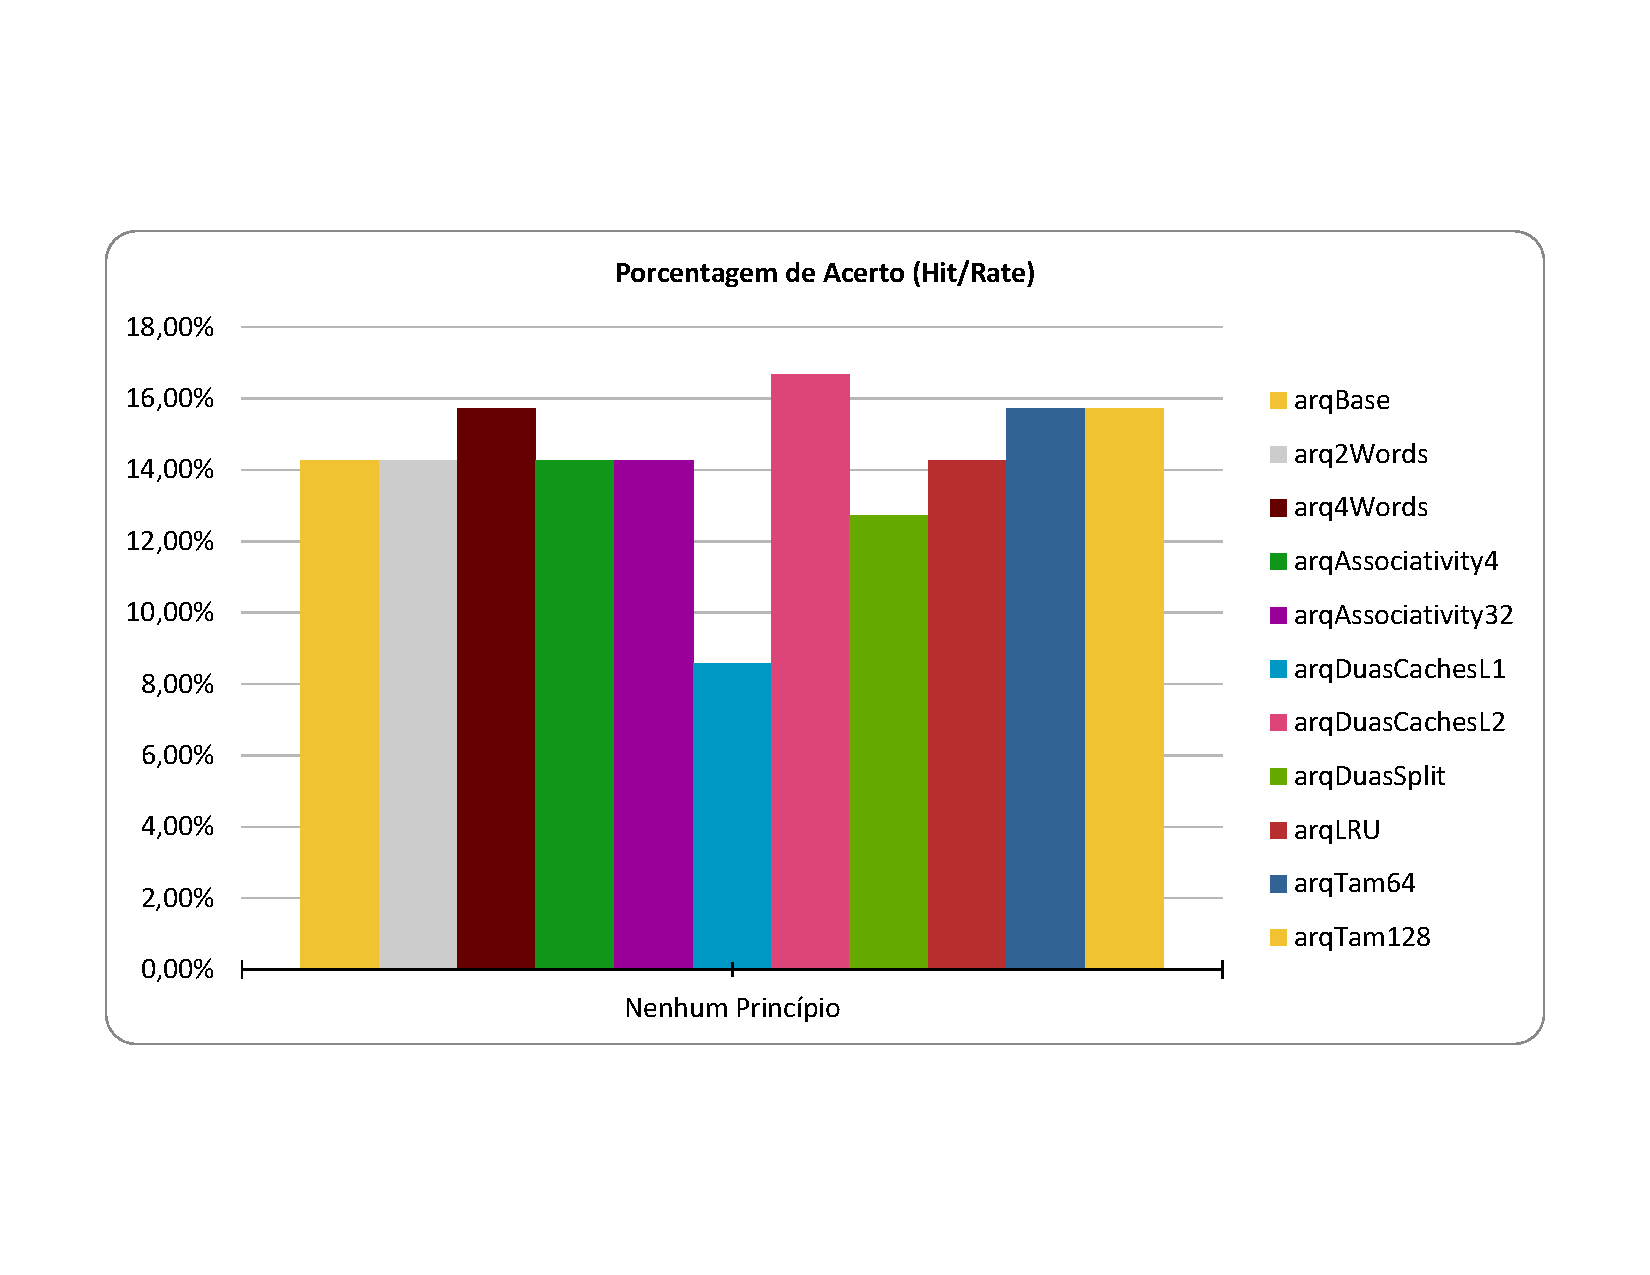
\includegraphics[width=\textwidth]{Random.pdf}
\end{figure}
\end{minipage}
\vspace{-1.5cm}
\subsubsection{Relação da taxa de acerto (hit rate) com o tamanho da cache}
O trace aleatório não respeita nenhum princípio de localidade espacial ou temporal, sendo assim esperado uma variação mínima na taxa de acerto. Nota-se que o tamanho da cache pouco influencia, uma vez que não é garantido um novo acesso em uma posição com o dado procurado. Como a ram possui 256 palavras, e a chance de se acessar uma mesma palavra duas vezes é baixa no trace aleatório, o aumento da cache pouco altera o resultado.
\subsubsection{Relação da taxa de acerto (hit rate) com o tamanho do bloco}
O aumento de hit$\backslash$rate para 4 palavras acontece apenas pelo fato de aumentar a chance de localidade espacial. Para 2 palavras não houve alteração pois não há nenhum acesso próximo o suficiente de um mesmo dado.
\subsubsection{Relação da taxa de acerto (hit rate) com o nível de associatividade}
Era de se esperar que para associatividade maior houvesse uma taxa maior de acertos, porém isso não acontece devido ao não respeito à nenhum princípio, uma vez que o aumento da associatividade melhora a localidade temporal.
\subsubsection{Relação da taxa de acerto (hit rate) com o algoritmo de substituição}
A mudança de algoritmo de substituição mostra que apenas quando um (ou ambos) os princípios são respeitados que elas fazem diferença. No caso de acessos aleatórios, não temos a garantia que um endereço será acessado repetidamente, para que o LRU seja mais eficaz, por exemplo.
\subsubsection{Relação da taxa de acerto (hit rate) com o número de caches}
O aumento de caches melhora, de fato, a taxa de acerto das escritas, onde foi obtido maior taxa de acerto. Já para a split, mais uma vez não temos garantia que, mesmo utilizando uma cache apenas para instruções, iremos reutilizar certas instruções. Além disso, ao fazer uma escrita, temos uma maior chance de não ter utilizado o mesmo endereço para escrita na cache de dados.
\section{Conclusão}
Sempre que pelo menos um dos princípios é respeitado, temos a possibilidade de melhorar a taxa de acerto utilizando uma arquitetura de cache onde já se espera o aumento do hit$\backslash$rate. Como a maioria dos programas hoje utilizados respeitam pelo menos um dos princípios, podemos sempre estimar uma arquitetura de cache que se melhor adequará às necessidades de tais programas, aumentando sua eficiência.
\end{document}